%!TEX root = ../Thesis.tex

\chapter{Nomenclature}
\begin{acronym}[TDMA]
\acro{CACHET}{Copenhagen Center for Health Technology} 
\acro{MDD}{Major Depressive Disorder} 
\acro{BA}{Behavioural Activation} 
\end{acronym}

\textbf{Major Depressive Disorder (MDD)}\\
Also known simply as depression, is a mental disorder characterized by low mood, low self-esteem, loss of interest in normally enjoyable activities, low energy, and pain without a clear cause.\\

\textbf{Behavioural Activation (BA)}\\
A therapeutic intervention that is often used to treat MDD. BA treatment focuses on keeping depression at bay through activities which produce positive reinforcement for the patient. BA is highly customizable and is a very personal treatment plan.\\

\textbf{Mobility}\\
How a person changes location over time.\\

\textbf{Mobility Feature}\\
A number which describes one of the ways in which a person changes location over time. Many features will paint a more complete picture of the mobility patterns than fewer features.\\



\chapter{Installation Manual}
\label{appendix:installation}
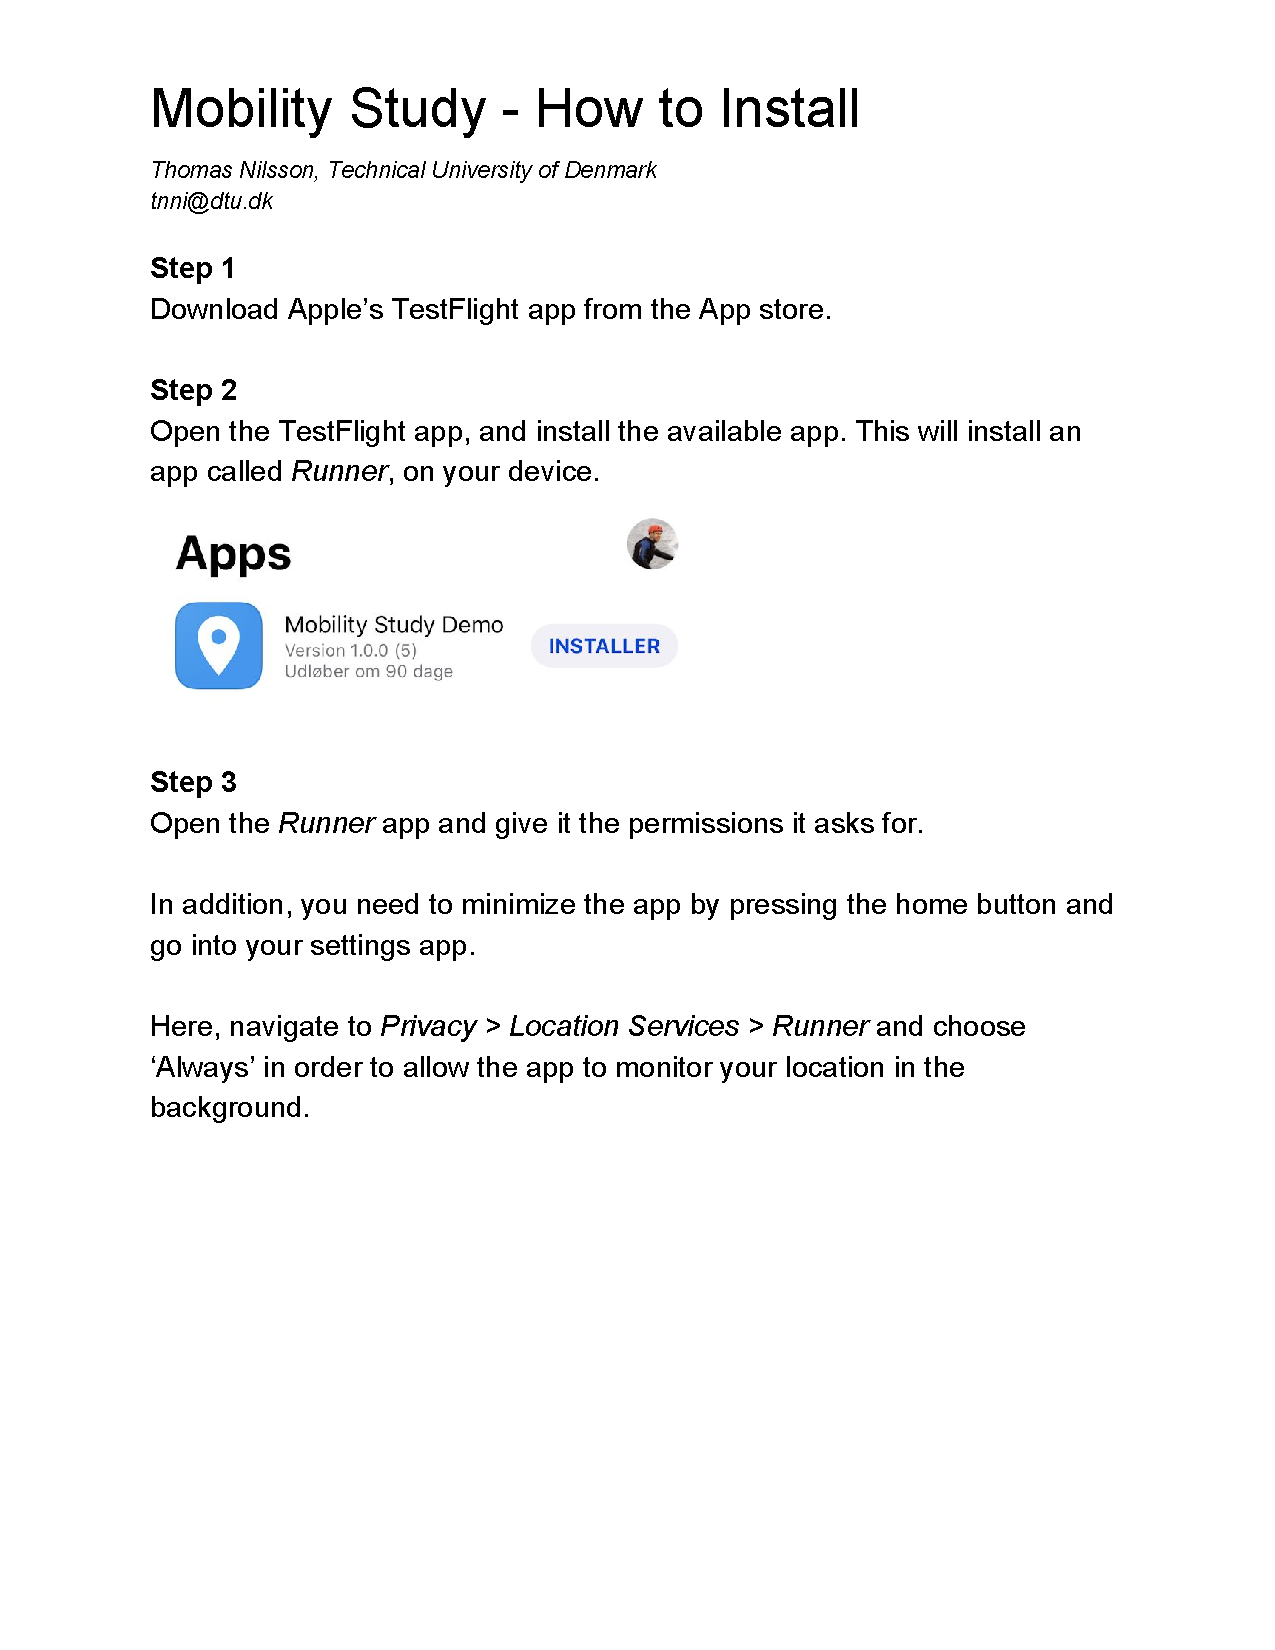
\includepdf[pages=-,pagecommand={},width=\textwidth]{appendices/installation.pdf}

